\documentclass[a4paper,10pt]{article}
\usepackage[paper=a4paper, left=1.5cm, right=1.5cm, bottom=2.0cm, top=1.6cm]{geometry}
%\usepackage[spanish]{babel}
\usepackage[spanish, es-noshorthands]{babel}
\usepackage[utf8]{inputenc}
\usepackage{color}
\usepackage{amsthm}

\usepackage{tikz}
\usetikzlibrary{arrows}


\usepackage{verbatim}
\usepackage{caratula1}
\usepackage{algorithm}
\usepackage{algpseudocode}
\usepackage{verbatim}
\usepackage{amsfonts}
\usepackage{amsmath}
\usepackage{graphicx}
%\usepackage{epstopdf}
\usepackage{ifpdf}
\usepackage{multicol}
\usepackage{caption}
\usepackage{subcaption}
%\usepackage{subfig}

\renewcommand{\algorithmicwhile}{\textbf{Mientras}}
\renewcommand{\algorithmicfor}{\textbf{Para}}
\renewcommand{\algorithmicif}{\textbf{Si}}
\renewcommand{\algorithmicthen}{\textbf{entonces}}
\renewcommand{\algorithmicelse}{\textbf{Si no}}
\renewcommand{\algorithmicdo}{}
\renewcommand{\algorithmicend}{\textbf{Fin}}
\renewcommand{\algorithmicreturn}{\textbf{Devolver}}
%\renewcommand{\algorithmicendif}{\algorithmicelse\ \algorithmicif}
\renewcommand{\cos}{\mathtt{c}}


\newcommand{\algorithmicendfor}{}
\newcommand{\algorithmicendwhile}{}
\newcommand{\algorithmicendif}{}
%\newcommand{\algorithmicprocedure}{}

%\renewcommand{\algorithmicendwhile}{\tetbf{fin mientras}}

\newcommand{\seno}{\mathtt{s}}
\newcommand{\R}{\mathbb{R}}
\newcommand{\N}{\mathbb{N}}
\newcommand{\inc}{\subseteq}
\newcommand{\eps}{\varepsilon}
\renewcommand{\O}{\mathcal{O}}

%\newcommand{\algorithmicto}{\textbf{a}}
\newtheorem{lema}{Lema}[subsection]
\newtheorem{prop}{Proposici\'on}[subsection]
\newtheorem{cor}[lema]{Corolario}


%este paquete es innecesario para el TP, acá lo uso para recuadrar
%\usepackage{framed}


\begin{document}
%Datos para la caratula
\materia{Métodos Num\'ericos}

\titulo{Trabajo Pr\'actico 3}

\subtitulo{}

\grupo{Grupo 14}

\integrante{Dabbah, Juli\'an}{015/09}{djulius@gmail.com}
\integrante{Dahlquist, Ariel}{383/10}{ariel.dahlquist@gmail.com}
\integrante{Garrone, Javier}{151/10}{javier3653@gmail.com}

\maketitle
\tableofcontents

\newpage
\section{Introducción}
En este T.P. deberemos decidir si la estructura de un puente, con ciertas cargas dadas, es estable. En este caso, analizaremos la estructura de puentes \emph{Prat Truss}, escribiendo las ecuaciones de fuerzas que se aplican sobre ciertas partes de la estructura. Luego resolveremos este sistema lineal y verificaremos que ninguna de los valores de fuerza obtenidos superen un límite determinado por los materiales de construcción. Para resolver el sistema utilizaremos el método de Eliminación de Gauss, al que aplicaremos algunas optimizaciones que permite este problema en particular, al igual que para la representación de la matriz en memoria. 

\subsection{Puentes \emph{Pratt Truss}}
Un esquema de puente \emph{Pratt Truss} puede verse en la figura \ref{fig:puente}.
\begin{figure}[!ht]
\begin{center}
\begin{tikzpicture}[scale = 0.7]

    \tikzset{nodestyle/.style={draw,shape=circle,scale=0.5}}
    \node[nodestyle] (p1) at ( 0, 0) {}; 
    \node[nodestyle] (p2) at ( 3, 0) {};
    \node[nodestyle] (p3) at ( 6, 0) {};
    \node[nodestyle] (p4) at ( 9, 0) {};
    \node[nodestyle] (p5) at ( 12, 0) {};
    \node[nodestyle] (p6) at ( 15, 0) {};
    \node[nodestyle] (p7) at ( 18, 0) {};

    \node[nodestyle] (p8) at ( 3, 2) {};
    \node[nodestyle] (p9) at ( 6, 2) {};
    \node[nodestyle] (p10) at ( 9, 2) {};
    \node[nodestyle] (p11) at ( 12, 2) {};
    \node[nodestyle] (p12) at ( 15, 2) {};

    \begin{scope}[every path/.style={-}]
        \draw (p1) -- (p2);
        \draw (p2) -- (p3); 
        \draw (p3) -- (p4);
        \draw (p4) -- (p5);
        \draw (p5) -- (p6);
        \draw (p6) -- (p7);

        \draw (p8) -- (p9);
        \draw (p9) -- (p10);
        \draw (p10) -- (p11);
        \draw (p11) -- (p12);

        \draw (p1) -- (p8);
        \draw (p12) -- (p7);

        \draw (p2) -- (p8);
        \draw (p3) -- (p9);
        \draw (p4) -- (p10);
        \draw (p5) -- (p11);
        \draw (p6) -- (p12);

        \draw (p8) -- (p3);
        \draw (p9) -- (p4);
        \draw (p4) -- (p11);
        \draw (p5) -- (p12);
    \end{scope}  

        \draw[fill=gray] (0.3,-0.15) rectangle (-2,-2);
        \draw[fill=gray] (17.7,-0.15) rectangle (20,-2);

    \node (c1) at ( 3, -2) {$c_1$};
    \node (c2) at ( 6, -2) {$c_2$};
    \node (c3) at ( 9, -2) {$c_3$};
    \node (c4) at ( 12, -2) {$c_4$};
    \node (c5) at ( 15, -2) {$c_5$};
    \draw[->] (p2) -- (c1);
  	\draw[->] (p3) -- (c2);
   	\draw[->] (p4) -- (c3);
    \draw[->] (p5) -- (c4);
    \draw[->] (p6) -- (c5);
\end{tikzpicture}
\caption{Esquema de la estructura de un puente \emph{Pratt Truss}. \small{(Cortesía Enunciado TP2)}}
\label{fig:puente}
\end{center}
\end{figure}

Dado que realizaremos el análisis únicamente en dos dimensiones (supondremos que las cargas se distribuyen uniformemente en la profundidad), pensaremos de ahora en más en esquemas como éste. Llamaremos \emph{link} a cada uno de los miembros de los que se compone la estructura, \emph{junta} a los puntos donde éstos se unen y \emph{sección} a la porción contenida entre dos links verticales sucesivos. Para el análisis en el T.P. trabajaremos con una cantidad par de secciones y supondremos que las cargas (y las fuerzas en general) se aplican únicamente sobre las juntas. Consideraremos como variables de la estructura la cantidad de secciones ($n$), la altura del puente ($h$), y la luz que debe cubrir ($span$). Podemos ver (como se muestraen la figura \ref{fig:estructuras}) que una estructura de $n$ secciones cuenta con $2n$ juntas y $4n-3$ links.

\begin{figure}[!ht]
\begin{center}
\begin{tikzpicture}[scale = 0.7]

    \tikzset{nodestyle/.style={draw,shape=circle,scale=0.5}}
    \node[nodestyle] (p1) at ( 0, 0) {}; 
    \node[nodestyle] (p2) at ( 3, 0) {};
    \node[nodestyle] (p3) at ( 6, 0) {};
    \node[nodestyle] (p4) at ( 9, 0) {};
    \node[nodestyle] (p5) at ( 12, 0) {};
    \node[nodestyle] (p6) at ( 15, 0) {};
    \node[nodestyle] (p7) at ( 18, 0) {};

    \node[nodestyle] (p8) at ( 3, 2) {};
    \node[nodestyle] (p9) at ( 6, 2) {};
    \node[nodestyle] (p10) at ( 9, 2) {};
    \node[nodestyle] (p11) at ( 12, 2) {};
    \node[nodestyle] (p12) at ( 15, 2) {};

    \begin{scope}[every path/.style={-}]
        \draw (p1) -- (p2) node[midway,above] {$S1$};
        \draw (p2) -- (p3) node[midway,above] {$S2$}; 
        \draw (p3) -- (p4) node[midway,above] {$S3$};
        \draw (p4) -- (p5) node[midway,above] {$S4$};
        \draw (p5) -- (p6) node[midway,above] {$S5$};
        \draw (p6) -- (p7) node[midway,above] {$S6= Sn$};

        \draw (p8) -- (p9);
        \draw (p9) -- (p10);
        \draw (p10) -- (p11);
        \draw (p11) -- (p12);

        \draw (p1) -- (p8);
        \draw (p12) -- (p7);

        \draw (p2) -- (p8);
        \draw (p3) -- (p9);
        \draw (p4) -- (p10);
        \draw (p5) -- (p11);
        \draw (p6) -- (p12);

        \draw (p8) -- (p3);
        \draw (p9) -- (p4);
        \draw (p4) -- (p11);
        \draw (p5) -- (p12);
    \end{scope}  

        \draw[fill=gray] (0.3,-0.15) rectangle (-2,-2);
        \draw[fill=gray] (17.7,-0.15) rectangle (20,-2);

        % Nodos artificiales.
        \node (a1) at ( 0, -3) {};
        \node (a2) at ( 18, -3) {};
        \node (a3) at ( -0.3, 0) {};
        \node (a4) at ( -0.3, 2) {};
        \node (a5) at ( 3, -0.5) {};
        \node (a6) at ( 6.3, -0.5) {};
		\node (c1) at ( 3, -2) {$c_1$};
    \node (c2) at ( 6, -2) {$c_2$};
    \node (c3) at ( 9, -2) {$c_3$};
    \node (c4) at ( 12, -2) {$c_4$};
    \node (c5) at ( 15, -2) {$c_5  = c_{n-1}$};
    \draw[->] (p2) -- (c1);
  	\draw[->] (p3) -- (c2);
   	\draw[->] (p4) -- (c3);
    \draw[->] (p5) -- (c4);
    \draw[->] (p6) -- (c5);        
        
        
        \begin{scope}[every path/.style={-}]
            \draw[dashed] (a1) -- (a2) node[below,midway]{$span$} ;
            \draw[dashed] (a3) -- (a4) node[left,midway]{$h$};
            \draw[dashed] (a5) -- (a6) node[below,midway]{$span/n$};
        \end{scope}
        
\end{tikzpicture}
\caption{Variables a considerar de la estructura, $n = 6$. \small{(Cortesía Enunciado TP2)}}
\label{fig:estructuras}
\end{center}
\end{figure}


Para asegurar la estabilidad, requeriremos que la fuerza resultante sobre cada junta sea nula. Es decir, que las fuerzas horizontales y verticales (y la descomposición en estas direcciones de las fuerzas oblicuas) se anulen en cada junta. Para satisfacer esto, consideraremos, por cada junta, una ecuación en dirección horizontal y otra en vertical, cuyas incógnitas serán las fuerzas ejercidads por los links. Construyendo esto para todas las juntas, tendremos un sistema de $4n$ ecuaciones. Si consideramos una variable por la fuerza ejercida por cada link tendremos $4n-3$ variables, a las que agregaremos fuerzas verticales sobre las juntas de los extremos y una fuerza horizontal sobre uno de éstos, para modelar la interacción del terreno, tendremos un sistema cuadrado de $4n$. Observemos que la cantidad de fuerzas que se ejercen sobre cada link es una cantidad constante (y pequeña) en relación al tamaño de la estructura, con lo cual, la mayoría de los coeficientes de las incógnitas serán nulos, generando una matriz muy esparsa.

\subsection{Representación Matricial}
Dado que las variables involucradas en cada ecuación son pocas, la matriz asociada al sistema resulta con una gran cantidad de coeficientes nulos, lo que nos motivó a utilizar una estructura de datos que aproveche este hecho, antes que la implementación trivial como arreglo bidimensional. Más aún, veremos que la matriz resultante tiene estructura de bandas, y que nuestro algoritmo de eliminación la conserva, con lo cual durante toda la vida de la matriz, sigue siendo considerablemente esparsa, con lo cual las ventajas siguen siendo válidas. En esta representación, decidimos almacenar las filas como listas enlazadas ordenadas por índice creciente, conteniendo únicamente elementos no nulos. La matriz, entonces, resulta en un vector de $n$ filas, en la cual, si bien el acceso aleatorio al elemento $i,j$ es más costoso que en el caso del arreglo bidimensional, las operaciones por filas tienen el mismo costo que en aquél y evitan considerar operaciones entre valores nulos.

\subsubsection{Matriz Banda}
Formalmente, decimos que una matriz $A \in \R ^{n\times n}$ tiene estructura de bandas $p,q$ si $a_{i,j} = 0$ cuando $j \leq i-p$ ó $j\geq i+q$, $1\leq i,j \leq n$.

\begin{lema}
Sea $A \in \R^{n \times n}$, con estructura de bandas $p, q$. Luego, en el peor de los casos, en todos los pasos del algoritmo de Eliminación Gaussiana con pivoteo parcial, la matriz resultante tiene estructura de bandas $p, q+p$
\end{lema}
\begin{proof}
Porque yo lo digo.
\end{proof}

\subsection{Algoritmo de Resolución}
Como dijimos, utilizaremos el método de Eliminación de Gauss, al que le agregaremos pivoteo parcial  ya que no podemos asegurar que éste no sea necesario en las condiciones de la matriz. Más allá de esto, no realizamos mayores modificaciones al algoritmo, únicamente aprovechar la existencia de la banda inferior para reducir el alcance de la búsqueda del pivote, ya que por debajo de ésta sólo encontraría ceros.





\section{Desarrollo}
	\subsection{Métodos propuestos}
%decir que son métodos mixtos. Que nos gusta la bisección porque nos asegura convergencia en caso de que lo necesitemos y porque no mete errores de propagación	
	Según lo consignado en el enunciado, exponemos a continuación los distintos métodos propuestos para computar $\frac{1}{\sqrt{\alpha}}$
	%Métodos generales -> Demostrar Newton, convergencia.
		\subsubsection{Cero de $f(x) = x^2 -\alpha$}
		Una alternativa propuesta en el enunciado consiste en calcular primero $\sqrt{\alpha}$ como un cero de la función $f(x) = x^2 -\alpha$, y luego calcular su inverso multiplicativo. Para esto utilizaremos el método de Newton (\ref{prop_newton}). Con lo cual, para encontrar un cero de $f$ debemos buscar un punto fijo de 
		\begin{equation}
			g(x) = x - \frac{f(x)}{f'(x)} = x - \frac{x^2 - \alpha}{2x} = \frac{x + \frac{\alpha}{x}}{2}
		\label{g}	
		\end{equation}
lo cual realizaremos construyendo la sucesión
	\begin{eqnarray}
		&& x_0 \in [a,b], \sqrt{\alpha} \in [a,b] \nonumber \\
		&& x_{n+1} = g(x_n) 
		\label{sqrtNewt}
	\end{eqnarray}
cuya convergencia dependerá de los valores de $a,b$. 

Demostramos el siguiente resultado teórico:

\begin{prop} [Convergencia del Método (Ej 3.a)]
Sea $\{x_n\}_{n\in\N}$ definida como en \ref{sqrtNewt}. Si $x_0 > \sqrt{\alpha}$, la sucesión converge cuadráticamente a $\sqrt{\alpha}$.
\begin{lema}
$x_n > \sqrt{\alpha}$ para cualquier $ n \geq 0$
\begin{proof}
Observemos primero la siguiente equivalencia:
$$x_{n+1} = \displaystyle \frac{1}{2} (x_{n} + \frac{\alpha}{x_{n}}) < x_n \Leftrightarrow \displaystyle \frac{1}{2} (1 + \frac{\alpha}{x^2_{n}}) < 1 \Leftrightarrow \frac{\alpha}{x_n^2} < 1 \Leftrightarrow \sqrt{\alpha} < x_n$$

Veamos que efectivamente se verifica que todos los términos de la sucesión están acotados inferiormente por $\sqrt{\alpha}$. Sabemos que los términos se construyen como $x_{n+1} =  \frac{x_n + \frac{\alpha}{x_n}}{2} = g(x_n)$, con lo cual veamos que podemos acotar inferiormente a $g$.

$$g(x) > \sqrt{\alpha} \Leftrightarrow \frac{1}{2}(x + \frac{\alpha}{x}) > \sqrt{\alpha} \Leftrightarrow  \alpha > -x^2 + 2x\sqrt{\alpha} \Leftrightarrow  0 > -x^2 + 2x\sqrt{\alpha} - \alpha \Leftrightarrow  0 < x^2 - 2x\sqrt{\alpha} + \alpha = (x-\sqrt{\alpha})^2$$  

Observando el signo de la desigualdad, al tratarse de un cuadrado, si el binomio no se anula, podemos afirmar la cota. Es decir:
$$g(x) > \sqrt{\alpha} \Leftrightarrow x \neq \sqrt{\alpha}$$

 Veamos que efectivamente esto no sucede para la sucesión, por inducción en $n$. Para $n = 0$, por hipótesis sabemos $x_0 > \sqrt{\alpha}$, con lo cual la diferencia no es nula. Para $x_n$, con $n\geq 1$ tenemos $x_n = g(x_{n-1})$. Como $x_{n-1}\neq \sqrt{\alpha}$ por hipótesis inductiva, se sigue$  \sqrt{\alpha} < g(x_{n-1}) = x_n$, como necesitábamos ver.
\end{proof}
\end{lema}
\begin{proof}
Veamos, ahora sí, que efectivamente el método converge. Para eso, veremos que se satisfacen las hipótesis del lema \ref{lema_f}.
\begin{description}
	\item[Derivabilidad] La función obtenida es continua y derivable en los reales estrictamente positivos, con lo cual esto se satisface en todos los intervalos sobre los que se trabajará.
	\item[Derivada acotada]  Necesitamos $g'(x) \leq k < 1$, con lo cual veamos $g'(x) = \frac{1}{2} (1- \frac{\alpha}{x^2})$. Sabemos ya que $x > \sqrt{\alpha}$, con lo cual, $ 0<\frac{\alpha}{x^2} < 1$, o sea $0 < g'(x) < \frac{1}{2}$.
	\item[Preservación del intervalo] Necesitamos $g([a,b]) \inc [a,b]$. Sabemos que $g$ puede tener un extremo en $\sqrt{\alpha}$, pues se anula su derivada primera. Miremos $g''(x) = \frac{\alpha}{x^3}$ para comprobarlo. Esta función es estrictamente positiva en $\R_{>0}$, con lo cual efectivamente se trata de un extremo y un mínimo. Además, podemos ver que si $x > \sqrt{\alpha}$ la derivada es positiva, y por lo tanto, la función creciente. Con lo cual, sea $\eps$  tal que $g(\sqrt{\alpha}) \leq g(x) \forall x\in [\sqrt{\alpha}-\eps, \sqrt{\alpha}-\eps]$, condición que sabemos que sucede por tratarse de un extremo local, sea $b > \sqrt{\alpha}$. Luego, $g([a,b]) = [g(\sqrt{\alpha}), g(b)]$, ya que, como la función es estrictamente creciente a la derecha del mínimo, el valor máximo lo alcanzará en el valor máximo de $x$, y por ser continua, tomará todos los valores intermedios entre su máximo y su mínimo. Ya sabemos $a = \sqrt{\alpha} -\eps < g(\sqrt{\alpha}) = \sqrt{\alpha}$, falta ver $g(b) < b$, pero imaginando $b = x_0$, esto vale por el lema anterior.
	
\end{description}
\end{proof}

\end{prop}
Además de esto, utilizamos otro argumento teórico para establecer un intervalo donde el método converja con seguridad. 
 Miremos ahora $ g'(x) = \frac{1}{2} - \frac{\alpha/2}{x^2}$.\\
$$ |g'(x)| = |\frac{1}{2} - \frac{\alpha/2}{x^2}|  < 1  
\Leftrightarrow  -1 < \frac{1}{2} - \frac{\alpha/2}{x^2} < 1 
	\Leftrightarrow  -\frac{3}{2} <  - \frac{\alpha/2}{x^2}  < \frac{1}{2}  \Leftrightarrow 3 >  \frac{\alpha}{x^2}  
	\Leftrightarrow  \frac{\sqrt{\alpha}}{\sqrt{3}} < x $$\\
Antes que nada, observemos que descartamos una de las desigualdades pues se cumple siempre por los signos de las expresiones. También sabemos $1/\sqrt{3} < 0.58 + \eps$, con lo cual tomando $x > 0.58\sqrt{\alpha} > \sqrt{\alpha}/\sqrt{3} + \eps'$ se verfica lo que necesitamos. Además, nuestro intervalo debe contener a $\sqrt{\alpha}$, con lo cual siempre vale $a \leq \sqrt{\alpha} \leq b$, por lo que si tomamos $a = 0.58b$ tenemos lo siguiente:
$$x \geq a \Leftrightarrow x \geq 0.58b \geq 0.58\sqrt{\alpha} \Rightarrow x > \sqrt{\alpha}/\sqrt{3} + \eps$$ 
como necesitábamos. 

Veamos ahora $g([a,b]) \inc [a,b]$. Observemos que $g$ tiene un único extremo en $\sqrt{a}$ y éste es un mínimo, pues $g'(\sqrt{\alpha}) = \frac{1}{2} - \frac{1}{2}\frac{\alpha}{(\sqrt{\alpha})^2} = \frac{1}{2} - \frac{1}{2}\frac{\alpha}{\alpha} = 0$ y además $g''(x) = \frac{\alpha}{x^3} >0$ para cualquier $x>0$. Luego, como se trata de unafunción continua, $g([a,b]) = [\sqrt{\alpha}, \max(g(a), g(b))]$. Siempre suponemos que $\sqrt{\alpha}\in[a,b]$, con lo cual basta asegurar $\max(g(a), g(b))\leq b$ para conseguir lo deseado.

Utilizaremos este último argumento ya que nos provee una forma explícita para los extremos, además de que se presta para ir obteniéndolos por sucesivas bisecciones desde un intervalo original, fácil de determinar. Como dijimos, de todas formas, sabemos que este proceso puede ser costoso en cuanto a tiempos, por lo que, experimentalmente, terminaremos de establecer cotas para los extremos, o limitar su cantidad de iteraciones.

		\subsubsection{Cero de $e(x) = \frac{1}{x^2} - \alpha$ - M\'etodo de Newton}
		La segunda alternativa es considerar a la función $e(x) = \frac{1}{x^2} - \alpha$ y buscar una aproximación a una de sus raíces: $\frac{1}{\sqrt{\alpha}}$, el valor que precisamente queríamos calcular en primera instancia. Para aproximar dicha raíz, planteamos dos métodos. El primero es aplicar el método de Newton para la función $e(x)$. Entonces, como vinimos explicando, buscamos hallar un punto fijo para la función
		\begin{equation}
			g(x) = x - \frac{e(x)}{e'(x)} = x - \frac{\frac{1}{x^2} - \alpha}{\frac{-2}{x^3}} = x + \frac{x - \alpha x^3}{2} = \frac{3x - \alpha x^3}{2}
		\label{g_e}
		\end{equation}
analizando la convergencia de la sucesión
		\begin{eqnarray}
		  && x_0 \in [a,b], \frac{1}{\sqrt{\alpha}} \in [a,b] \nonumber \\
		  && x_{n+1} = g(x_n) \nonumber
		\end{eqnarray}
		
Nuevamente, para asegurar la convergencia, buscamos un intervalo $[a,b]$ que satisfaga las hipótesis del Lema \ref{lema_f}.
  En primer lugar, $g(x)$ está bien definida, es continua y derivable en el intervalo $(0, +\infty)$ por ser un polinomio. Como mencionamos anteriormente, $\frac{1}{\sqrt{\alpha}}$ no está definida para $\alpha \leq 0$, con lo cual asegurar continuidad y derivabilidad en $(0,+\infty)$ es suficiente.\\
  
  Analicemos $|g'(x)| = |\frac{3}{2} - \frac{3}{2}\alpha x^2|$:\\\\
  $$
	 |g'(x)| < 1 
	 \Leftrightarrow |\frac{3}{2} - \frac{3}{2}\alpha x^2| < 1 
	 \Leftrightarrow -1 < \frac{3}{2} - \frac{3}{2}\alpha x^2 < 1
	 \Leftrightarrow \frac{1}{3\alpha} < x^2 < \frac{5}{3\alpha}
	 \Leftrightarrow \frac{1}{\sqrt{3}\sqrt{\alpha}} < x < \frac{\sqrt{5}}{\sqrt{3}\sqrt{\alpha}} \mbox{ siempre } x > 0
$$
  Ahora consideremos $0 < \alpha < 1$, esto implica que $\alpha < \sqrt{\alpha}$ y $\sqrt{\alpha} < \frac{1}{\alpha} \Leftrightarrow \alpha < \frac{1}{\sqrt{\alpha}}$.  Luego, 
$$      \frac{1}{\sqrt{3}\sqrt{\alpha}} < x < \frac{\sqrt{5}}{\sqrt{3}\sqrt{\alpha}} \Leftrightarrow \frac{\alpha}{\sqrt{3}} < x < \sqrt{\frac{5}{3}}\frac{1}{\alpha} \\
$$ 
  Por otro lado, si $\alpha \geq 1$, $\alpha \geq \sqrt{\alpha} \Leftrightarrow \alpha \geq \frac{1}{\sqrt{\alpha}}$. Para este caso podemos afirmar entonces:
	  $$	      \frac{1}{\sqrt{3}\sqrt{\alpha}} < x < \frac{\sqrt{5}}{\sqrt{3}\sqrt{\alpha}} \Leftrightarrow \frac{1}{\sqrt{3}\alpha} < x < \sqrt{\frac{5}{3}}\alpha $$
	  
Realizaremos un análisis similar al anterior para asegurar $g([a,b]) \inc [a,b]$. Sea $p = \frac{1}{\sqrt{\alpha}}$, miremos $g'(x) = \frac{3-3\alpha x^2}{2}$. Ya sabemos $g'(p) = 0$, miremos $g''(p) =  -3 \alpha x$, que es estrictamente negativa en los números positivos, y por lo tanto, el punto crítico es un máximo. Con un argumento similar al que utilizamos en métodos anteriores, sabemos $g([a,b]) \inc [min(g(a), g(b)), p]$. Podemos ver que $g(x) > x$ para cualquier $0<x<\frac{1}{\alpha}$, con lo cual ya tenemos $g(a) > a$. También se puede deducir fácilmente que $g(b) \leq b$, tanto para cualquiera de los dos casos del valor de $\alpha$.


\subsubsection{Cero de $e(x) = \frac{1}{x^2} - \alpha$ - Punto fijo}
Además de buscar esta raíz con el método de Newton, propusimos otra función cuyo punto fijo sea el cero buscado. Comenzamos tomando $g(x) = \frac{1}{\alpha} \frac{1}{x}$, que tiene un punto fijo en  $p = \frac{1}{\sqrt{\alpha}}$ y $e(p)= 0$. Sin embargo, $g'(x) = -\frac{1}{\alpha} \frac{1}{x^2}$ no se anula en $p$, con lo cual su orden de convergencia es lineal. Dado que ya contábamos con un método cuadrático, decidimos transformar $g$ para obtener convergencia cuadrática anulando su derivada primera. Planetamos lo siguiente: sea $h = g + t \cdot s$, siendo $t(p) = 0$. Por un lado, esto garantiza que $p$ sea punto fijo de $h$, ya que $h(p) = g(p) + t(p)s(p) = g(p) + 0\cdot s(p) = g(p) = p$, y por otro nos resultaría fácil de encontrar, ya que habíamos considerado múltiples funciones que se anulan en el punto buscado. Mejor aún es cómo hace que se comporte $h$ al derivarla: $h' = g' + t'\cdot s + t \cdot s'$, que evaluado en $p$ resulta: $h'(p) = g'(p) + t'(p)s(p) + 0\cdot s'(p) = g'(p) + t'(p)s(p)$, lo cual elimina cualquier restricción posible sobre la derivada de $s$. Propusimos $t(x) = e(x)$, con lo cual, resulta $h'(p) = g'(p) + e'(p)s(p) = 1 + e'(p)s(p)$. Si queremos $h'(p) = 0$ basta pedir $e'(p)s(p) = -1$, que se satisface fácilmente tomando $s = \frac{-1}{e'}$. Siendo $e'(x) = \frac{-2}{x^3}$, tenemos $s(x) = \frac{x^3}{2}$.

Finalmente, tenemos 
\begin{equation}
	h(x) = \frac{1}{\alpha} \frac{1}{x} + (\frac{1}{x^2} - \alpha)\frac{x^3}{2} =  \frac{1}{\alpha x} + \frac{x - \alpha x^3}{2}
\end{equation}
que, por cómo la construimos, convergerá cuadráticamente cuando le apliquemos el método de punto fijo.

En este caso no demostraremos el intervalo de convergencia, simplemente procedemos a ajustar el intervalo bisectando la derivada, hasta que en ambos extremos se verifique $|g'(x)| < 1$.

\subsubsection{Bisección de $x^2-\alpha$}
Aprovechando que ya teníamos implementado el procedimiento de bisección, lo aplicamos a buscar el cero de $f(x) = x^2-\alpha$. La implementaión es trivial y no merece mayor comentario, lo utilizaremos únicamente para comparar contra los otros resultados.



\subsection{//UN TÍTULO PARA ESTO}
	
Como expusimos anteriormente (OBVIO), en todos los casos en que aplicamos el método de Newton tenemos argumentos teóricos para asegurar su convergencia en orden cuadrático, a costo de reducir iterativamente por bisección un intervalo dentro del cual que podamos asegurar que la raíz buscada existe hasta que satisfaga las hipótesis del lema. Aprovecharemos esta garantía para fijar el criterio de parada de los métodos, una vez definido el cual y conociendo el desempeño del algoritmo en un caso teóricamente óptimo nos dedicaremos a relajar los parámetros que aseguran convergencia para determinar, experimentalmente, cotas para éste que representen mejor un compromiso entre calidad de la solución y tiempo de ejecución.

	\subsubsection{Función de control}
Para medir la calidad de la solución, implementamos la función $f(x) = \frac{1}{\sqrt{x}}$ directamente sobre el hardware, mediante una pequeña rutina de lenguaje ensamblador. Ésta utiliza únicamente las funciones cociente y raíz cuadrada del procesador, con lo cual confiamos en que, si bien también es una aproximación, es una de las mejores aproximaciones que podemos esperar dada la máquina.

	\subsubsection{Criterio de parada}
Establecimos como principal criterio de parada un umbral para el error relativo entre iteraciones sucesivas. Además, agregamos una condición de corte por cantidad de iteraciones para evitar problemas en eventuales casos patológicos que no hayamos contemplado en este análisis. Para determinar el umbral, realizaremos nuestras aproximaciones para las raíces pedidas tomando varios valores de $\alpha$ dentro de distintos órdenes de magnitud, repitiendo esto para distintos órdenes de magnitud de tolerancia. Luego, promediaremos los errores relativos de las soluciones dentro de cada orden de magnitud, a partir de lo cual compararemos los resultados obtenidos para las distintas tolerancias <redactame>, buscando, por un lado, descartar sobreexigencias, es decir, tolerancias <redactame> muy pequeñas que no aporten significativamente a la calidad de la solución, a la vez que otras que, aunque tal vez lo hagan, impliquen excesivo tiempo de cómputo. Este último caso será el más difícil de determinar, y de darse nos 
obligará a realizar nuevos experimentos para establecer el compromiso entre calidad y eficiencia.

	\subsubsection{Performance}
Como comentamos en la sección anterior (OBVIO), nuestros métodos cuentan con dos etapas: una en la cual ajustan un intervalo alrededor de la raíz mediante sucesivas bisecciones y otra donde efectivamente aplican un método iterativo de orden de convergencia mayor. Sabemos que la condición expresada en el lema \ref{lema_f} es suficiente pero no necesaria, con lo cual probablemente sea excesivamente exigente en la práctica. De todas maneras, un intervalo pequeño hace que los métodos cuadráticos converjan en muy pocas iteraciones, con lo cual no nos parece una mala idea invertir iteraciones tratando de ajustar las cotas iniciales si esto se verá reflejado en la cantidad de iteraciones que necesitará el método cuadrático para converger.

Para determinar este balance comenzaremos observando cuántas iteraciones realiza cada parte del algoritmo para valores que produzcan intervalos iniciales particularmente grandes, y cómo varía esta proporción a medida que se restringen las primeras. Una vez conocido esto (en principio, a grandes razgos), mediremos el tiempo que efectivamente tardan en computarse, ya que no podemos suponer que los dos tipos de iteraciones sean igual de costosos computacionalmente. Teniendo esta variable en mente, realizaremos el mismo tipo de ajustes que planteamos antes <redactame>.

	\subsubsection{Comparación final}
Una vez ajustados los mejores parámetros de cada método en base a los valores obtenidos experimentalmente, compararemos los métodos entre sí. Además de los aspectos que ya comentamos para cada método por separado, compararemos las aproximaciones obtenidas por cada uno sobre una batería de casos (EEEEPA), donde pretendemos diferenciar su desempeño (tanto en calidad de la solución como en velocidad de cómputo) para diferentes valores de entrada, eligiendo éstos especialmente para poner a prueba diferentes debilidades posibles (intervalo inicial muy grande, inestabilidad numérica (EEEEPA), etc), así como también sobre valores aleatorios dentro de un rango suficientemente grande para considerarlo representativo de uso. Con estos datos intentaremos establecer cuál es el método más conveniente para utilizar, y si esto depende y cómo de los valores de entrada.



\newpage
\section{Resultados}

\subsection{Criterio de Parada}
Realizamos, para cada método, las mediciones comentadas en la sección anterior, obteniendo los siguientes resultados.
\begin{figure}[H]
  \centering
    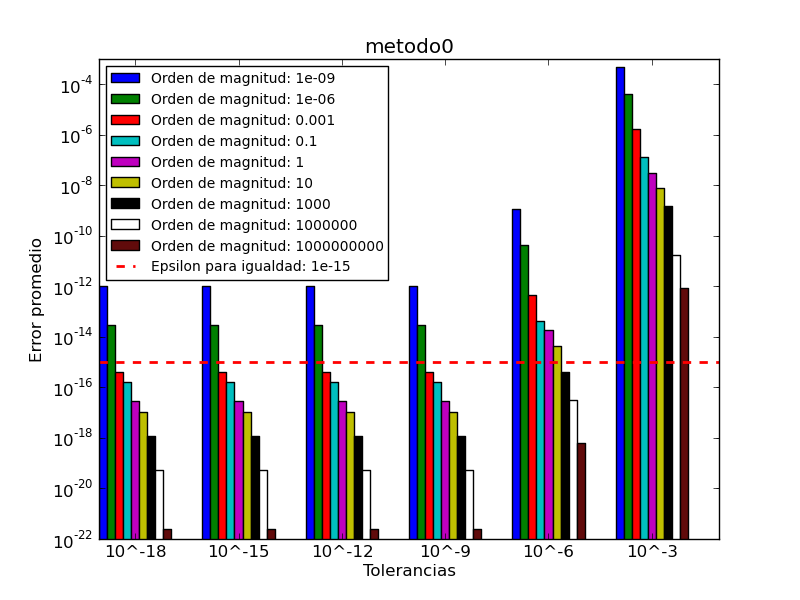
\includegraphics[width=0.9\textwidth]{../data/metodo0.png}
    \caption{Error relativo final para distintos valores de tolerancia en el criterio de parada utilizando el cero de $x^2-\alpha$ con el método de Newton para cada orden de magnitud medido.}
    \label{paradaMet0}
\end{figure}

Para el primer método, calculamos $z^{-1}$, siendo $z$ un cero de $f(x) = x^2-\alpha$ que obtuvimos mediante el método de Newton. En la figura \ref{paradaMet0} vemos el error relativo final (luego de calculado el cociente) según las distintas tolerancias. Observamos, por un lado, que todos los errores decrecen (no estrictamente) a medida que decrece la tolerancia, lo cual es esperable. Por otro lado, observamos un estancamiento del error para $\tau < 10^{-9}$, con lo cual éste será el valor elegido para este método. Si bien es llamativo que el error no se reduzca para tolerancias menores, sabiendo que el método converge cuadráticamente podemos pensar que el error relativo del criterio de parada se reduce, en una iteración de un valor en el orden de $10^-6$ a uno por debajo de $10^-18$, haciendo que el método termine para todas las tolerancias intermedias al mismo tiempo. Pensamos en investigar qué sucedería para tolerancias menores, pero dado que consideramos como iguales valores que difieran en menos de $10^{-15}$ consideramos que no tenía significación.

Observemos también que el error relativo se hace más significativo cuanto menor es el orden de magnitud, lo que indicaría que el error absoluto no necesariamente acompaña la magnitud de $\alpha$. Atribuimos esto a errores numéricos, que se introducen siempre independientemente del valor representado.


\begin{figure}[H]
  \centering
    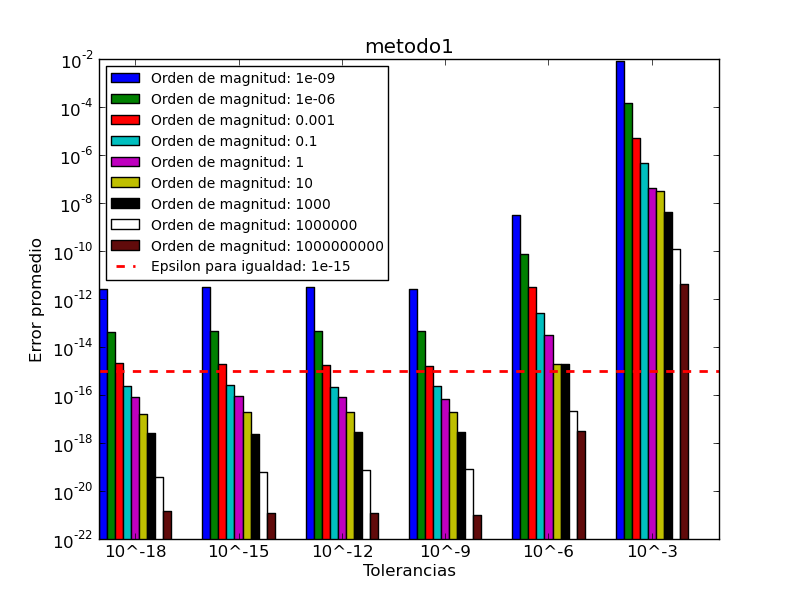
\includegraphics[width=0.9\textwidth]{../data/metodo1.png}
    \caption{Error relativo final para distintos valores de tolerancia en el criterio de parada para el cero de $\frac{1}{x^2} - \alpha$ con el método de Newton para cada orden de magnitud medido.}
    \label{paradaMet1}
\end{figure}

Observemos que el gráfico es muy similar al de la figura \ref{paradaMet1}, con lo cual, al tratarse del mismo método, caben argumentos similares: el decrecimiento y estancamiento lo atribuimos a la rapidez con la que converge el método y podemos utilizar $10^{-9}$ para el criterio de parada.

\begin{figure}[H]
  \centering
    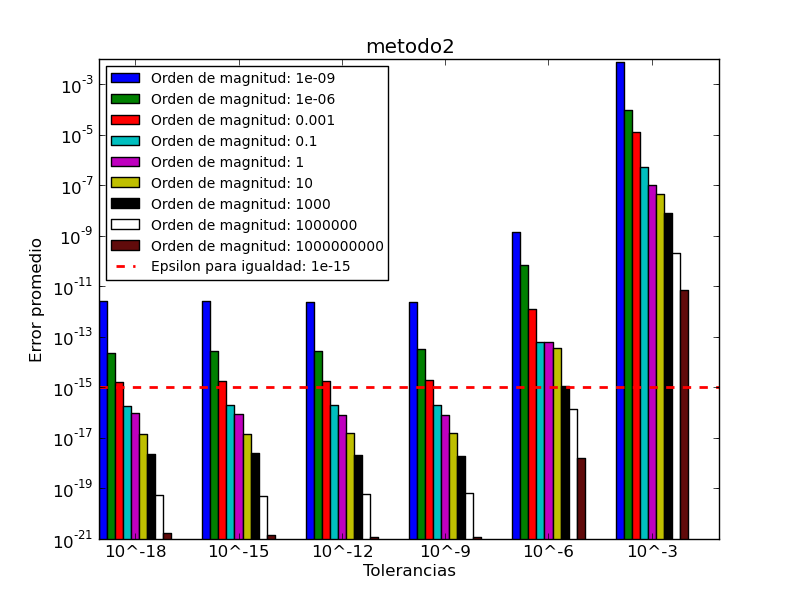
\includegraphics[width=0.9\textwidth]{../data/metodo2.png}
    \caption{Error relativo final para distintos valores de tolerancia en el criterio de parada para el cero de $\frac{1}{x^2} - \alpha$ con el método de punto fijo para $\frac{1}{\alpha x} + \frac{x - \alpha x^3}{2}$, para cada orden de magnitud medido.}
    \label{paradaMet2}
\end{figure}

Al igual que en el caso anterior, la figura \ref{paradaMet2}, al tratarse de un método cuadrático, admite un análisis análogo a los casos anteriores. En este caso también elegiremos $10^{-9}$.

\begin{figure}[H]
  \centering
    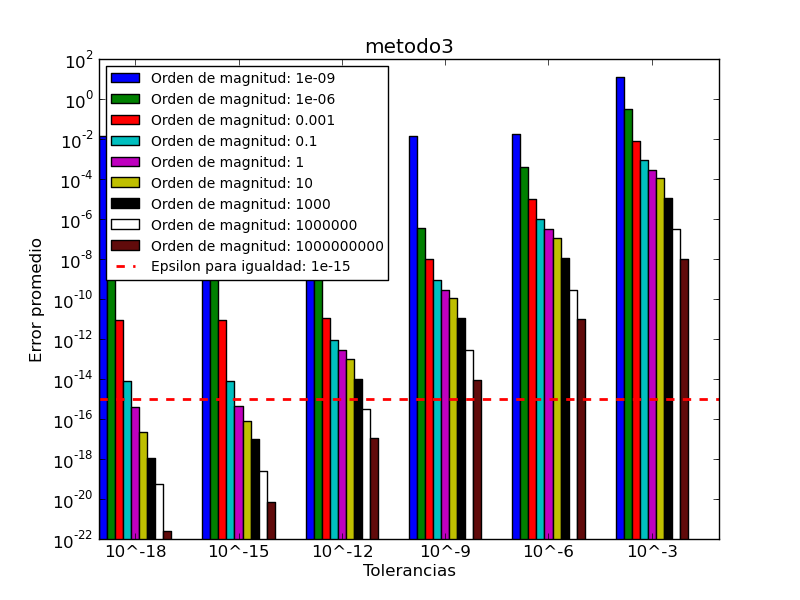
\includegraphics[width=0.9\textwidth]{../data/metodo3.png}
    \caption{Error relativo final para distintos valores de tolerancia en el criterio de parada obteniendo el cero de $x^2 - \alpha$ mediante bisección, para cada orden de magnitud medido.}
    \label{paradaMet3}
\end{figure}

Como dijimos, no esperábamos grandes resultados para este método. Elegiremos para seguir $10^{-15}$, que es donde se detiene la reducción del error (nuevamente, relacionado con el criterio de igualdad establecido). Vemos que para los órdenes más pequeños el error relativo es significativo, aún para las tolerancias menores, lo que indica que el error absoluto sigue siendo importante. Sabemos que para $\sqrt{\alpha}$ éste está acotado por la mitad de la longitud del intervalo en el último paso de bisección, que al calcularle el recíproco, tratándose de valores pequeños, éste crece considerablemente.

\subsection{Tiempo de Ejecución}

Para medir tiempo de ejecución, en principio, tomamos los métodos mixtos, sin restricciones sobre la cantidad de bisecciones. En general observamos que los tiempos crecen a medida que el orden de magnitud crece en módulo. Esto está relacionado con los intervalos inciales que elige cada método, que en general están en función de $\alpha$ o $\frac{1}{\alpha}$, según si se trata de valores mayores o menores a uno.
 
\begin{figure}[H]
  \centering
    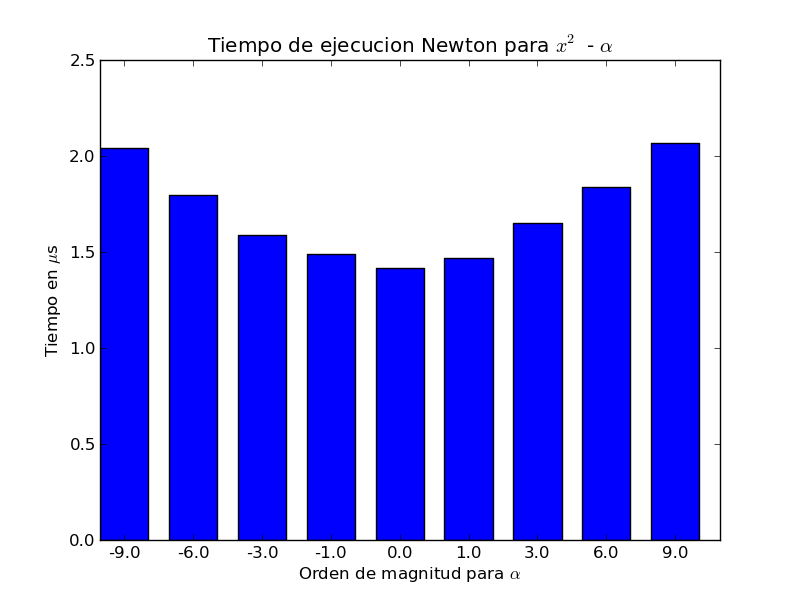
\includegraphics[width=0.9\textwidth]{../data/Tiempo metodo 0.png}
    \caption{Tiempo de ejecución para el recíproco del cero de $x^2 - \alpha$ con el método de Newton para cada orden de magnitud medido.}
    \label{tiempoMet0}
\end{figure}

Como dijimos, el tiempo de ejecución depende del orden de magnitud. Excepto en los casos extremos, la variación entre el mejor y el peor caso es perfectamente tolerable.

\begin{figure}[H]
  \centering
    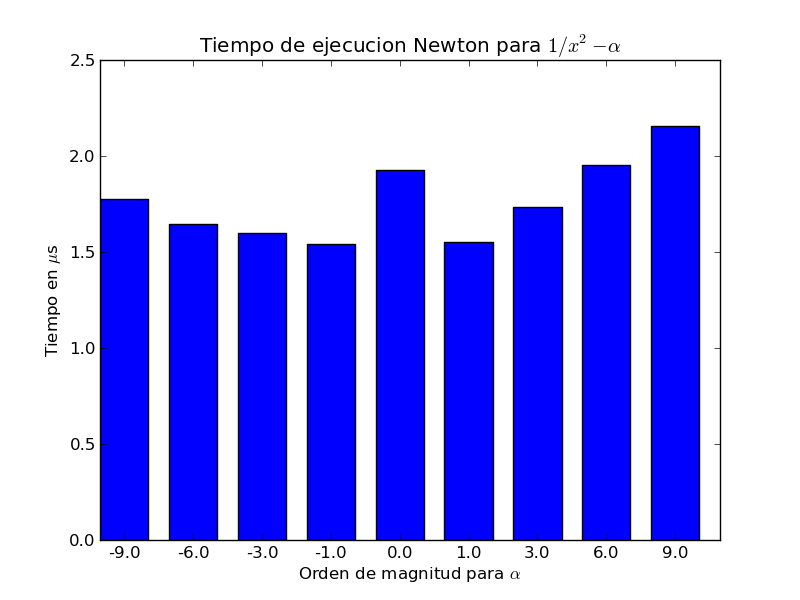
\includegraphics[width=0.9\textwidth]{../data/Tiempo metodo 1.png}
    \caption{Tiempo de ejecución para el cero de $\frac{1}{x^2} - \alpha$ con el método de Newton para cada orden de magnitud medido.}
    \label{tiempoMet1}
\end{figure}

//SI SE LES OCURRE ALGO PARA DECIR PARA EL PICO ALREDEDOR DEL 0 =)

\begin{figure}[H]
  \centering
    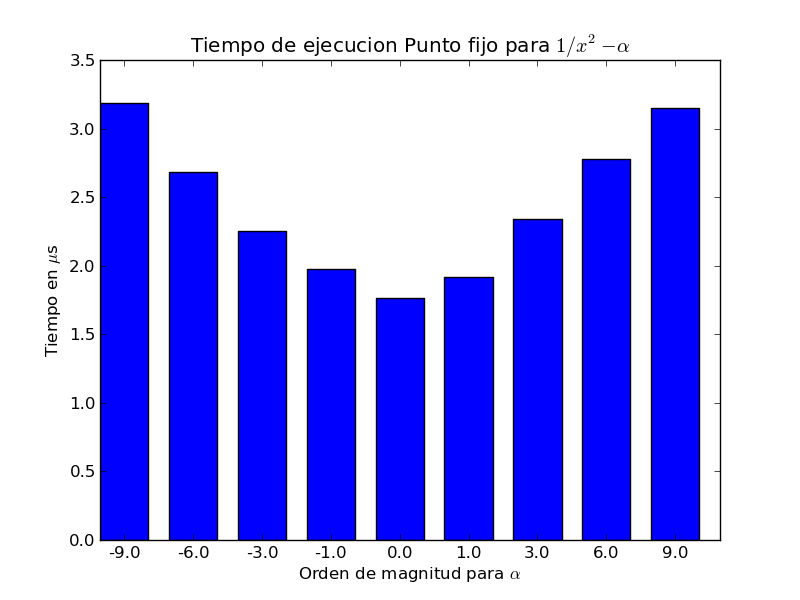
\includegraphics[width=0.9\textwidth]{../data/Tiempo metodo 2.png}
    \caption{Tiempo de ejecución para el cero de $\frac{1}{x^2} - \alpha$ con el método de punto fijo para cada orden de magnitud medido.}
    \label{tiempoMet2}
\end{figure}

Nuevamente, el tiempo depende del orden de magnitud en el que estamos calculando. Observamos una situación similar a la de la figura \ref{tiempoMet0}, aunque éste método parece más costoso. Esto es esperable si tenemos en cuenta que la función de punto fijo que utiliza contiene más operaciones que la que utilizamos para  el caso anterior.

\begin{figure}[H]
  \centering
    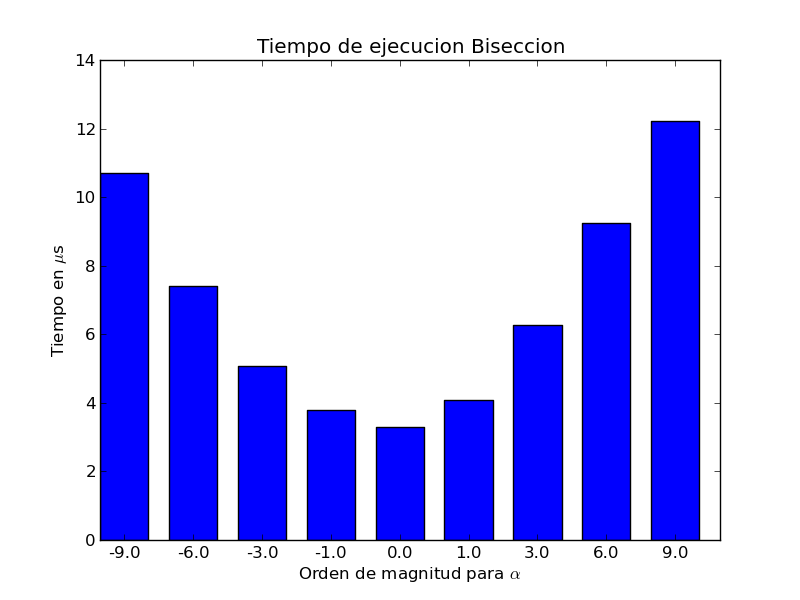
\includegraphics[width=0.9\textwidth]{../data/Tiempo metodo 3.png}
    \caption{Tiempo de ejecución para el recíproco del cero de ${x^2} - \alpha$ con bisección para cada orden de magnitud medido.}
    \label{tiempoMet3}
\end{figure}

Si bien observamos que la forma general del gráfico es similar a los casos anteriores, si miramos la escala vemos que se trata de un método mucho más lento. Esto es lo que esperábamos, ya que sabemos que converge linealmente, mientras que los otros métodos propuestos los elegimos por tener convergencia cuadrática.


%\input{discusion.tex}
%\section{Conclusiones}

Fijamos una tolerancia para cada método de acuerdo a las observaciones que pudimos hacer en base a los resultados: dicha tolerancia fue de ${10^-9}$ para
todos los métodos menos para bisección, ${10^-15}$ para esta última que es el $\epsilon$ que tomamos para evaluar cuándo dos número de punto flotante son iguales. A partir de dichos valores, la precisión de cada método se mantiene constante con una cota de error por debajo de ${10^-12}$.

En cuanto al tiempo de ejecución no pudimos observar grandes cambios de método a método, pero sin embargo es sencillo deducir las diferencias de tiempos basándonos en la operaciones que se computan en cada método. Para el primer método, el cuál calcula el inverso multiplicativo del cero de $f(x) = x^2 - \alpha$




En vista de los resultados, concluimos que el método de la bisección es que peor resultados nos trajo en relación a todos los parámetros que evaluamos (tolerancia de error, tiempo de ejecución y cantidad de iteraciones).
%\input{apendices.tex}
%\input{referencias.tex}


\end{document}
